\documentclass[11pt,letterpaper]{article}

%\usepackage{naaclhlt2013}
%\usepackage{times}
%\usepackage{latexsym}
%\setlength\titlebox{6.5cm}    % Expanding the titlebox


\usepackage{graphicx}
\usepackage{amsmath,amssymb}
\usepackage[english]{babel}
\usepackage[utf8]{inputenc}
\usepackage[ruled,vlined]{algorithm2e}
\usepackage{url}
\usepackage{float}%figure environment
\usepackage{multirow}
\usepackage{booktabs}
\usepackage{todonotes}
\usepackage{booktabs}
\usepackage{mdframed}
\usepackage{wrapfig}


\title{AGDISTIS - Agnostic Disambiguation of Named Entities Using Linked Open Data}

%\author{Ricardo Usbeck, Axel-Cyrille {Ngonga Ngomo}, \\
%        \textbf{S\"oren Auer, Daniel Gerber}\\
%	    University of Leipzig\\
%	    Augustusplatz 10\\
%	    04109 Leipzig, Germany\\
%	    {\tt$\{$usbeck$|$ngonga$|$auer$|$dgerber$\}$}\\
%	    {\tt{@}informatik.uni-leipzig.de}
%	  \And
%	Andreas Both\\
%  	R\,\&\,D, Unister~GmbH\\
%  	Barfussg\"asschen 11\\
%  	Leipzig, Germany\\
%  {\tt andreas.both@unister.de}
%}

\author{Author A, Author B, \\
        \textbf{Author C, Author D}\\
	    University X\\
	    Adress Y\\
	    TOWN Z\\
	    {\tt$\{$a$|$b$|$c$|$d$\}$}\\
	    {\tt{@}somewhere}
	  \And
	Author E\\
  	Company F\\
  	Adress M\\
  	Town N\\
  {\tt e@somewhereelse}
}

%\date{}

\begin{document}

%\maketitle
\newmdtheoremenv{ex}{Example}
 
\section*{Appendix - Algorithm for expansion policy}
\begin{algorithm}[h!]
\KwData{$N=\{N_1,N_2\dots N_n\}$ sorted in ascending order of their string length, trigram similarity threshold $\sigma$}
\KwResult{set of candidates $C$}
\Begin{
{\bf heuristicExpansion} $\longleftarrow \emptyset$, 
{\bf C}  $\longleftarrow \emptyset$ \;
\For{$N_i \in N$}{
    {\bf label} $\longleftarrow$ {\bf string(}$N_i${\bf)}\;
    {\bf tmp} $\longleftarrow$ {\bf label}\;
    {\bf expansion} $\longleftarrow$ {\bf false}\;
   \For{{\bf key} $\in$ {\bf  heuristicExpansion}}{ 
       \If{{\bf key} {\bf contains label}} {
            \If{{\bf tmp.length} $ > $ {\bf key.length} $\&\&$ {\bf tmp} $!=$ {\bf label}} {
                         {\bf tmp} $\longleftarrow$ {\bf key}\;
                         {\bf expansion} $\longleftarrow$ {\bf true}\;
                    }
             \If{{\bf tmp.length} $<$ {\bf key.length} $\&\&$  {\bf tmp} $==$ {\bf label}} {
                         {\bf tmp} $\longleftarrow$  {\bf key}\;
                         {\bf expansion} $\longleftarrow$ {\bf true}\;
                    }
            }}
            {\bf label} $\longleftarrow$ {\bf tmp}\;
            \If{$\neg${\bf expansion}} {
                {\bf heuristicExpansion} $\longleftarrow$ {\bf label} $\cup$  {\bf heuristicExpansion}
            }
          {\bf $C\longleftarrow C \cup$ searchCandidates(label,$\sigma$)}\;
}}
\caption{Search candidates for named entities and expansion policy\label{expandNE}}
\end{algorithm}

\clearpage
\begin{table*}[htb!]
\centering
\caption{Test corpora specifications}
\label{tab:data}
\begin{tabular}{lccccc}
\toprule
\textbf{Corpus} & \textbf{Language} & \textbf{{\#}Doc.} & \textbf{{\#}Ent.} & \textbf{Avg.(Ent./Doc.)}  & \textbf{Annotation }\\
\midrule
Reuters-21578  & English & 145 & 769 &5.30& voter agreement\\
RSS 500 & English & 500 & 1,000 & 2.00&domain expert \\
\url{news.de} & German & 53 & 627 & 11.83&domain expert \\
AIDA-YAGO2 & English & 1,393 & 34,956 &25.07&voter agreement\\
\bottomrule
\end{tabular}
\end{table*}
\section*{Results on other corpora with different KBs}
\begin{table*}[htb!]
\centering
\caption{Evaluation of AGDISTIS. Bold indicates best \mbox{F-measure}.} 
\begin{tabular}{c ccc ccc}
\toprule
\textbf{Corpus}  & \multicolumn{6}{c}{\textbf{AGDISTIS}}	\\\midrule
\textbf{Knowledge Base}& \multicolumn{3}{c}{{DBpedia}}& \multicolumn{3}{c}{{YAGO2}}\\\midrule
				& \mbox{F-measure} 		& $\quad \sigma \quad $ & $\quad d \quad $ 	& \mbox{F-measure} & $\quad \sigma \quad $ & $\quad d \quad $ \\
\cmidrule(r){2-4}  \cmidrule(r){5-7} 
Reuters-21578	&  	\textbf{0.78}	&  			0.87		&  		2			& 	0.60	&  0.29		&  	3	\\
RSS 500 		&  	\textbf{0.75}	&  			0.76		&  		2			& 	0.53	&  0.82		&   2 	\\
\url{news.de} 	&  	\textbf{0.87}	&  			0.71		&  		2			& 	---		&   ---		&  ----	\\
AIDA-YAGO2	   	&  		0.73		&  			0.89		&  		2			& 	0.58	&  0.76		&   2 	\\
\bottomrule
\end{tabular}
\end{table*}
\begin{table*}[htb!]
\centering
\caption{Evaluation of AGDISTIS against AIDA and DBpedia Spotlight. Bold indicates best \mbox{F-measure}.} 
\begin{tabular}{c  c c}
\toprule
\textbf{Corpus}  	& \textbf{AIDA} & \textbf{Spotlight}\\\midrule
\textbf{Knowledge Base}& {YAGO2} & {DBpedia}\\\midrule
				&  \mbox{F-measure}  & \mbox{F-measure}\\
\cmidrule{8-8} \cmidrule{9-9}
Reuters-21578	&  	0.62		& 	0.56	\\
RSS 500 		&  	0.60		& 	0.40	\\
\url{news.de} 	&  	----		& 	0.84	\\
AIDA-YAGO2	   	&\textbf{0.83}	& 	0.57	\\
\bottomrule
\end{tabular}
\end{table*}

\clearpage

\section*{Appendix - Figures of experimental results}
\begin{figure}[htb!]
    \centering
        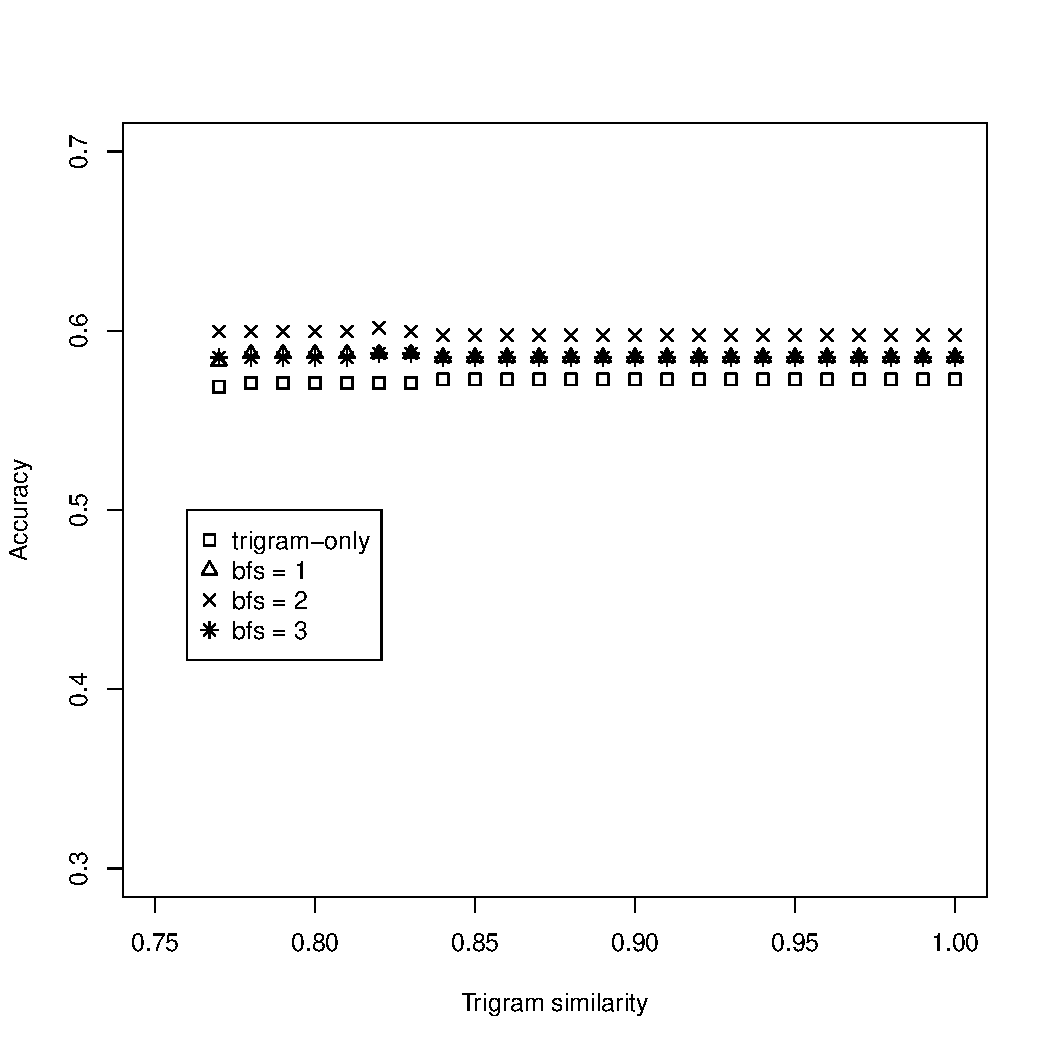
\includegraphics[width=\linewidth]{fig/500news.pdf}
    \caption{Accuracy of AGDISTIS on the \textbf{RSS 500} corpus.}\label{fig:RSS500}
\end{figure}
\begin{figure}[htb!]    
    \centering  
         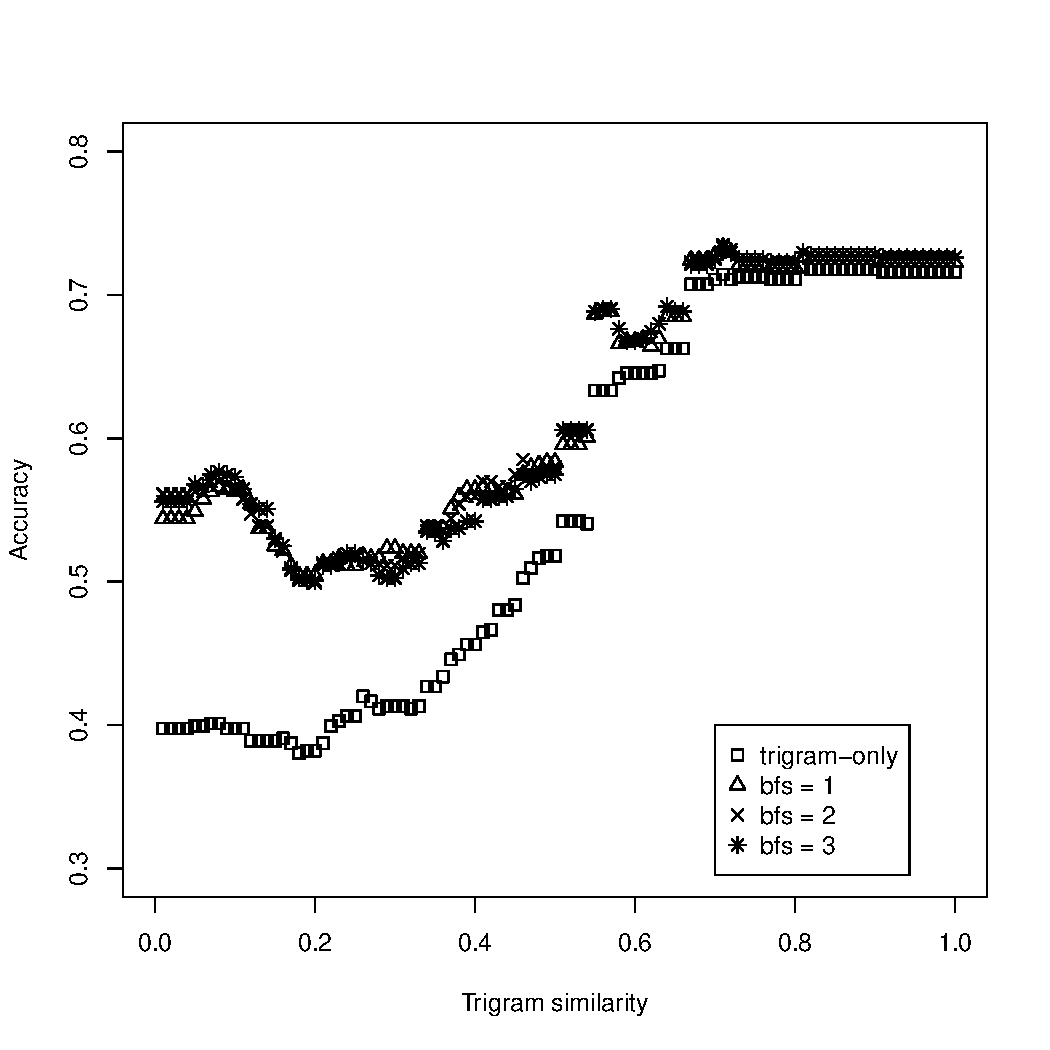
\includegraphics[width=\linewidth]{fig/german.pdf}
    \caption{Accuracy of AGDISTIS on the \textbf{news.de} corpus.}\label{fig:german} 
\end{figure}
\begin{figure}[htb!]    
    \centering  
         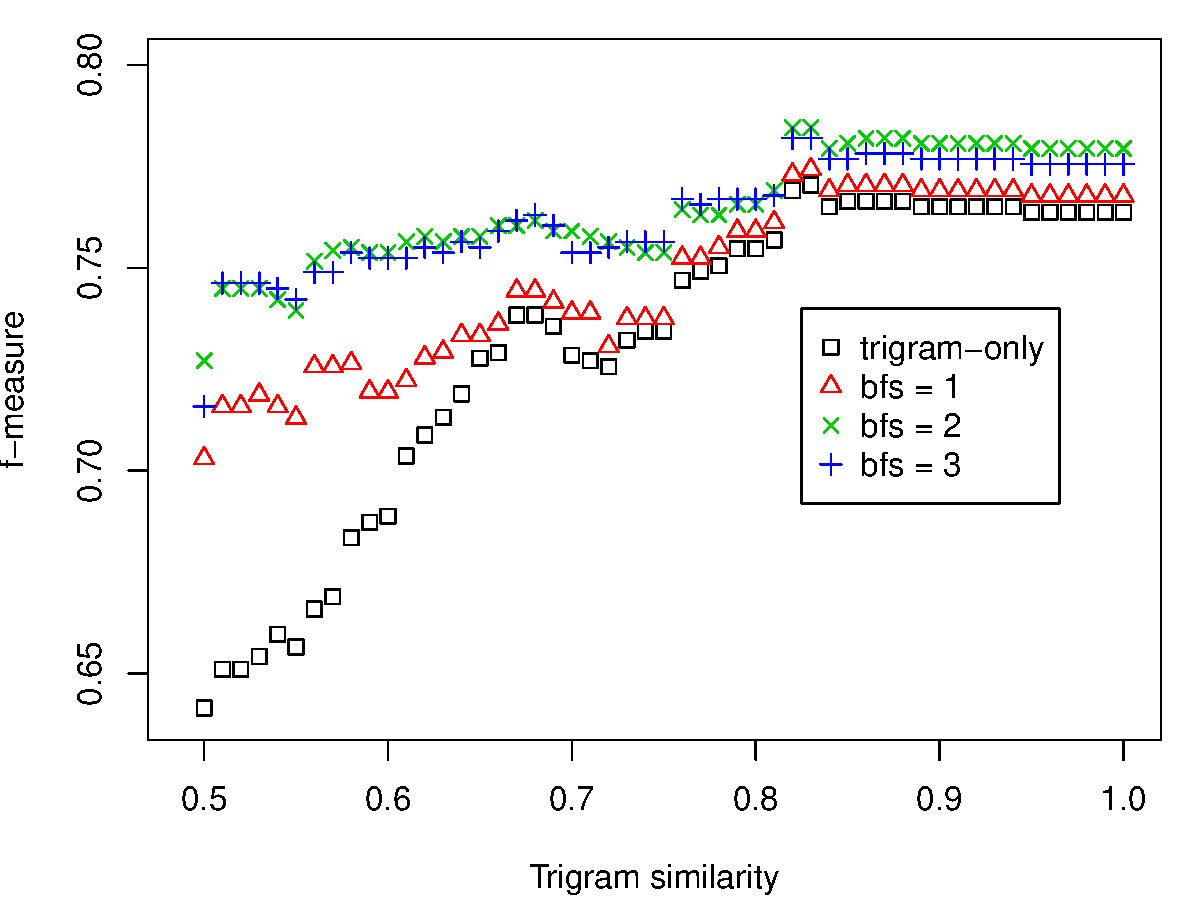
\includegraphics[width=\linewidth]{fig/reuters.pdf}
    \caption{Accuracy of AGDISTIS on the \textbf{reuters.de} corpus.}\label{fig:reuters} 
\end{figure}
\begin{figure}[htb!]    
    \centering  
         \includegraphics[width=\linewidth]{fig/runtimes.pdf}
    \caption{Comparison of the average runtime of AGDISTIS and AIDA on Reuters-21578 corpus with respect to the number of entities per sentence. AGDISTIS is cleary more time-efficient than AIDA.}\label{fig:runtimeVSentities} 
\end{figure}

\begin{figure}[htb!]    
    \centering  
         \includegraphics[width=\linewidth]{fig/surface.pdf}
    \caption{Influence of surface forms.} 
\end{figure}
\section*{Appendix - Quality Rater Tool}

\begin{figure}[htb!]    
    \centering  
         \includegraphics[width=\linewidth]{fig/qrtoolnew.png}
    \caption{Quality Rater Tool.} 
\end{figure}
%\clearpage
%\section*{Appendix - Effect of cumulatively removing properties}
%\begin{table}[htb!]
%\centering
%\scriptsize
%\caption{Effect of cumulatively removing properties, trigram similarity threshold $\sigma=0.835$, Reuters-21578, $d=2$, Prefix: dbpedia-owl.}
%\begin{tabular}{p{0.85\linewidth}c}
%\textbf{Property}  & \textbf{Accuracy}\\
%\toprule
%owner & 0.675\\\midrule
%isPartOf & 0.672\\\midrule
%countySeat & 0.670\\\midrule
%city & 0.666\\\midrule
%owningCompany, party, hometown, religion, memberOfParliament, occupation, influencedBy, locationCity, type, deputy, aircraftHelicopter, spouse, usingCountry, architect, knownFor, place, residence, governor, industry, timeZone, influenced, league, division, deathPlace, team, populationPlace, keyPerson, bandMember, operatedBy, officialLanguage, broadcastNetwork, march, education, season, regionalLanguage, battle, aircraftRecon, stylisticOrigin, militaryUnit, predecessor, wikiPageDisambiguates, leaderFunction, youthWing, derivative, fourthCommander, nationality, leaderParty, languageRegulator, leftTributary, parentCompany, language, country, militaryBranch, mayor, athletics, languageFamily, formerBandMember, largestCity, programmeFormat, state, location, territory, musicSubgenre, affiliation, aircraftTransport, associatedBand, garrison, primeMinister, part, otherParty, restingPlace, locationCountry, currency, aircraftElectronic, foundationPlace, related, neighboringMunicipality, award, relation, chairman, foundedBy, distributingLabel, isPartOfMilitaryConflict, colour, secondCommander, commander, ideology, lieutenant, formerTeam, broadcastArea, product, commandStructure, child, ground, routeStart, headquarter, spokenIn, profession, musicFusionGenre, recordLabel, anthem, successor, notableCommander, regionServed, governingBody, operator, service, hubAirport, militaryRank, aircraftTrainer, president & 0.664\\\midrule
%parent, jurisdiction, vicePresident, district, genre, pictureFormat, capital, birthPlace, region, governmentType, leaderName, leader, ethnicGroup, targetAirport, campus, monarch, thirdCommander, subsidiary, twinCity, almaMater, instrument, internationalAffiliation & 0.661\\\midrule
%managerClub, manager & 0.663\\\midrule
%sisterStation & 0.664\\\bottomrule
%\end{tabular}
%\label{tab:propertyEval}
%\end{table}

\end{document}

